\chapter{Differentiable manifolds} \label{s:man}

\minitoc

\section{Introduction}

Starting from basic mathematical definitions, we present
the implementation of manifolds and coordinate charts in \Sage{}
(Sec.~\ref{s:bas:manif}).
We then focus on the algebra of scalar fields on a manifold~\eqref{s:man:scalar_field_algebra}.
As we shall see in Chap.~\ref{s:vec}, this algebra plays a central role in the implementation of vector fields, the latter being considered as forming a module
over it.

\section{Differentiable manifolds} \label{s:bas:manif}

\subsection{Topological manifolds} \label{s:bas:def_manif}

Let $\K$ be a topological field. In most applications $\K=\R$ or $\K=\mathbb{C}$.
Given an integer $n\geq 1$, a \defin{topological manifold of dimension $n$ over $\K$}\index{manifold}\index{dimension of a manifold} is a topological space $\M$ obeying the following properties:
\begin{enumerate}
\item $\M$ is a \defin{separated space}\index{separated space} (also called \defin{Hausdorff space}\index{Hausdorff space}): any two distinct points of $\M$
admit disjoint open neighbourhoods.
\item $\M$ has a \defin{countable base}\index{countable base}:\footnote{In the language of topology, one says that $\M$ is a \emph{second-countable space}.}
there exists a countable family
$(U_k)_{k\in\mathbb{N}}$ of open sets of $\M$ such that any open set of $\M$ can be written as the union (possibly infinite) of some members of this family.
\item Around each point of $\M$, there exists a neighbourhood which is
homeomorphic to an open subset of $\K^n$.
\end{enumerate}
Property 1 excludes manifolds with ``forks''.
Property~2 excludes ``too large'' manifolds; in particular it permits setting
up the theory of integration on manifolds. In the case $\K=\R$, it also
allows for a smooth manifold of dimension $n$ to be embedded smoothly into the Euclidean space $\R^{2n}$
(Whitney theorem\index{Whitney theorem}).
Property~3 expresses the essence of a manifold: it means that, locally,
$\M$ ``resembles'' $\K^n$.

Let us start to discuss the implementation of manifolds in \Sage{}. We shall
do it on a concrete example, exposed in a Jupyter notebook which can be downloaded
from the page devoted to these lectures:
\begin{center}
\url{https://sagemanifolds.obspm.fr/jncf2018/}
\end{center}
As for all \Sage{}, the syntax used in this notebook is \soft{Python} one. However, no
a priori knowledge of \soft{Python} is required, since we shall explain the
main notations as they appear.

In \Sage{}, manifolds are constructed by means of the global function \code{Manifold}:

\begin{NBin}
%display latex
\end{NBin}

\begin{NBin}
M = Manifold(2, 'M')
print(M)
\end{NBin}
\begin{NBprint}
2-dimensional differentiable manifold M
\end{NBprint}
By default, the function \code{Manifold} returns a manifold over $\K=\R$:
\begin{NBin}
M.base_field()
\end{NBin}
\begin{NBoutM}
\mathbf{R}
\end{NBoutM}
Note the use of the standard object-oriented notation (ubiquitous in
\soft{Python}): the method \code{base\_field()} is called on the object \code{M};
since this method does not require any extra argument (all the information lies
in \code{M}), its argument list is empty, hence the final \code{()}.
Base fields different from $\mathbb{R}$
must be specified with the optional keyword \code{field}, like
\begin{flushleft}
\code{M = Manifold(2, 'M', field='complex')}
\end{flushleft}
We may check that $M$ is a topological space:
\begin{NBin}
M in Sets().Topological()
\end{NBin}
\begin{NBout}
\texttt{True}
\end{NBout}
Actually, $M$ belongs to the following categories:
\begin{NBin}
M.categories()
\end{NBin}
\begin{NBout}
\vspace{-25pt}  % manual hacking of the spacing; best I can do for right now -- TS
\begin{gather*}
\left[\mathbf{Smooth}_{\mathbf{R}}, \mathbf{Differentiable}_{\mathbf{R}}, \mathbf{Manifolds}_{\mathbf{R}}, \mathbf{TopologicalSpaces}(\mathbf{Sets}), \right.
\\ \left. \mathbf{Sets},  \mathbf{SetsWithPartialMaps}, \mathbf{Objects}\right]
\end{gather*}
\end{NBout}
As we can see from the first category in the above list, \code{Manifold}
constructs a smooth manifold by default.
If one would like to stick to the topological level, one should add
the keyword argument \code{structure='topological'} to \code{Manifold},
i.e.\ \code{M = Manifold(2, 'M', structure='topological')}: $M$ would have
been a topological manifold without any further structure.

\begin{figure}
\begin{center}
\begin{tikzpicture}[font=\small, node distance=0.5cm, minimum
height=2em, auto]

\node[native](unique_representation)
{\code{UniqueRepresentation}};

\node[native, right=of unique_representation](parent)
{\code{Parent}};

\coordinate (Middle) at ($(unique_representation)!0.5!(parent)$);

\node[diff, below=1.5cm of Middle](subset)
{\code{ManifoldSubset}\\ {\scriptsize {\it element:} \code{ManifoldPoint}}};
\path[line] (subset) -- (unique_representation);
\path[line] (subset) -- (parent);

\node[diff, below=of subset](manifold)
{\code{TopologicalManifold}};
\path[line] (manifold) -- (subset);

\node[diff, below=of manifold](diffmanifold)
{\code{DifferentiableManifold}};
\path[line] (diffmanifold) -- (manifold);

\node[diff, below=of diffmanifold](interval)
{\code{OpenInterval}};
\path[line] (interval) -- (diffmanifold);

\node[diff, below=of interval](realline)
{\code{RealLine}};
\path[line] (realline) -- (interval);

%
\node[native, right=1.5cm of parent](element)
{\code{Element}};

\node[diff, below=1.225cm of element](point)
{\code{ManifoldPoint}};

\path[line] (point) -- (element);

% legend

\node[native_legend, left=5cm of subset]
(native_legend){};
\node[empty, right=0.5em of native_legend]
{Generic \Sage{} class};

\node[diff_legend, below=1.em of native_legend]
(diff_legend){};
\node[empty, right=0.5em of diff_legend]
{\soft{SageManifolds} class\\ \footnotesize (differential part)};

\end{tikzpicture}

\end{center}
\caption{\label{f:man:domain_classes}\footnotesize
Python classes for topological
manifolds, differentiable manifolds, subsets of them
and points on them (\code{ManifoldPoint}).}
\end{figure}


Manifolds are implemented by the Python classes \code{TopologicalManifold}
and \\ \code{DifferentiableManifold} (see Fig.~\ref{f:man:domain_classes}),
actually by dynamically generated subclasses of those, via \Sage{} category
framework:\footnote{See \url{http://doc.sagemath.org/html/en/reference/categories/sage/categories/primer.html}\index{category} for details.}
\begin{NBin}
type(M)
\end{NBin}
\begin{NBout}
\begin{verbatim}
<class 'sage.manifolds.differentiable.manifold.
        DifferentiableManifold_with_category'>
\end{verbatim}
\end{NBout}
Notice that the actual class of \code{M} is \code{DifferentiableManifold-with-category}.
It is a subclass of \code{DifferentiableManifold}:
\begin{NBin}
isinstance(M,
           sage.manifolds.differentiable.manifold.DifferentiableManifold)
\end{NBin}
\begin{NBout}
\texttt{True}
\end{NBout}
and hence of
\code{TopologicalManifold} according to the inheritance diagram of Fig.~\ref{f:man:domain_classes}:
\begin{NBin}
isinstance(M, sage.manifolds.manifold.TopologicalManifold)
\end{NBin}
\begin{NBout}
\texttt{True}
\end{NBout}
Notice that \code{TopologicalManifold} itself is a subclass of \code{ManifoldSubset} (the class
for generic subsets of a manifold), which reflects the fact that $M\subset M$.

\subsection{Coordinate charts} \label{s:man:coord_chart}

Property~3 in the definition of a topological manifold (Sec.~\ref{s:bas:def_manif})
means that one can label the points of $\M$ in a
continuous way by $n$ numbers $(x^\alpha)_{\alpha\in\{0,\ldots,n-1\}}\in \K^n$,
which are called \defin{coordinates}\index{coordinate}.
More precisely, given an open subset $U\subset\M$, a \defin{coordinate chart}\index{coordinate!chart}
(or simply a \defin{chart}\index{chart})
on $U$ is a homeomorphism\footnote{Let us recall that a  \defin{homeomorphism}\index{homeomorphism} between two topological spaces
(here $U$ and $X(U)$) is a bijective map $X$ such
that both $X$ and $X^{-1}$ are continuous.}
\be \label{e:man:def_chart}
    \begin{array}{rccl}
    X: & U\subset \M & \longrightarrow & X(U)\subset \K^n \\
        & p & \longmapsto & (x^0, \ldots, x^{n-1}) .
    \end{array}
\ee
We declare a chart, along with the symbols used to denote the coordinates
(here $x=x^0$ and $y=x^1$) by
\begin{NBin}
U = M.open_subset('U')
XU.<x,y> = U.chart()
XU
\end{NBin}
\begin{NBoutM}
(U, (x,y))
\end{NBoutM}
Open subsets of a differentiable manifold are implemented by a (dynamically generated) subclass of
\code{DifferentiableManifold}, since they are differentiable manifolds in their own:
\begin{NBin}
isinstance(U,
           sage.manifolds.differentiable.manifold.DifferentiableManifold)
\end{NBin}
\begin{NBout}
\texttt{True}
\end{NBout}

Points on $M$ are created from their coordinates in a given chart:
\begin{NBin}
p = U((1,2), chart=XU, name='p')
print(p)
\end{NBin}
\begin{NBprint}
Point p on the 2-dimensional differentiable manifold M
\end{NBprint}
The syntax \code{U(...)} used to create $p$ as an element of $U$
reflects the parent/element\index{parent}\index{element} pattern employed in \Sage{}; indeed $U$
is the parent of $p$:
\begin{NBin}
p.parent()
\end{NBin}
\begin{NBoutM}
U
\end{NBoutM}
Points are implemented by a dynamically generated subclass of
\code{ManifoldPoint} (cf.\ Fig.~\ref{f:man:domain_classes}).
The principal attribute of this class is the one storing the point's coordinates
in various charts; it is implemented as
a Python dictionary,\footnote{A \defin{dictionary}\index{dictionary},
also known as \defin{associative array}, is a
data structure that generalizes the concept of array in the sense that the
key to access to an element is not restricted to an integer or a tuple of integers.} whose keys are the charts:
\begin{NBin}
p._coordinates
\end{NBin}
\begin{NBoutM}
\{(U, (x,y)): (1,2)\}
\end{NBoutM}
The leading underscore in the name \code{\_coordinates} is a notation
convention to specify that this attribute is a \defin{private} one:
the dictionary \code{\_coordinates} should
not be manipulated by the end user or involved in some code
outside of the class \code{ManifoldPoint}.
It belongs to the internal implementation, which may be changed while
the user interface of the class \code{ManifoldPoint} is kept fixed. We show
this private attribute here
because we are precisely interested in implementation features.
The public way to recover the point's coordinates is to let the chart act on
the point (reflecting thereby the definition~\eqref{e:man:def_chart} of a chart):
\begin{NBin}
XU(p)
\end{NBin}
\begin{NBoutM}
(1,2)
\end{NBoutM}

Usually, one needs more than a single coordinate system to cover $\M$.
An \defin{atlas}\index{atlas} on $\M$ is a set of pairs
$(U_i,X_i)_{i\in I}$, where $I$ is a set, $U_i$ an open set of $\M$ and $X_i$ a chart on $U_i$,
such that the union of all $U_i$'s covers $\M$:
\be
    \bigcup_{i\in I} U_i = \M.
\ee
Here we introduce a second chart on $\M$:
\begin{NBin}
V = M.open_subset('V')
XV.<xp,yp> = V.chart("xp:x' yp:y'")
XV
\end{NBin}
\begin{NBoutM}
\left( V, (x', y') \right)
\end{NBoutM}
and declare that $\M$ is covered by only two charts, i.e.\ that $M=U\cup V$:
\begin{NBin}
M.declare_union(U, V)
\end{NBin}
\begin{NBin}
M.atlas()
\end{NBin}
\begin{NBoutM}
\left[ \left(U, (x,y) \right), \left( V, (x', y') \right) \right]
\end{NBoutM}

\subsection{Smooth manifolds}

For manifolds, the concept of differentiability is
defined from the smooth structure of $\K^n$, via an atlas:
a \defin{smooth manifold}\index{smooth!manifold}\index{manifold!smooth --},
is a topological manifold $\M$ equipped with an atlas
$(U_i,X_i)_{i\in I}$ such that for any non-empty intersection
$U_i \cap U_j$, the map
\be \label{e:bas:transition_map}
    X_i \circ X_j^{-1} : X_j(U_i \cap U_j)
    \subset \K^n \longrightarrow X_i(U_i \cap U_j)
    \subset \K^n
\ee
is smooth (i.e.~$C^\infty$).
Note that the above map is from an open set of $\K^n$ to an open set of $\K^n$, so that the invoked differentiability is nothing but that of $\K^n$.
Such a map is called a \defin{change of coordinates}\index{change!of coordinates}\index{coordinate!change} or, in the mathematical literature, a
\defin{transition map}\index{transition map}.
The atlas $(U_i,X_i)_{i\in I}$ is called a
\defin{smooth atlas}\index{smooth!atlas}\index{atlas!smooth --}.

\begin{remark}
Strictly speaking a smooth manifold is a pair $(\M,\mathcal{A})$  where
$\mathcal{A}$ is a (maximal) smooth atlas on $\M$.
Indeed a given topological manifold $\M$
can have non-equivalent differentiable structures, as shown by Milnor (1956)~\cite{Milno56}
in the specific case of the unit sphere of dimension~7, $\mathbb{S}^7$: there exist smooth manifolds, the so-called \emph{exotic spheres}\index{exotic!sphere},
that are homeomorphic to $\mathbb{S}^7$ but not diffeomorphic
to $\mathbb{S}^7$.  On the other side, for $n\leq 6$, there is a unique smooth
structure for the sphere $\mathbb{S}^n$.
Moreover, any manifold of dimension $n\leq 3$ admits a unique smooth structure.
Amazingly, in the case of $\R^n$, there exists a unique smooth structure (the standard one) for any $n\not=4$, but for $n=4$ (the spacetime case!) there exist uncountably many non-equivalent smooth structures, the so-called
\emph{exotic $\R^4$}\index{exotic!$\R^4$}~\cite{Taube87}.
\end{remark}


For the manifold $M$ under consideration, we define the transition map \code{XU}~$\to$~\code{XV}
on $W = U\cap V$ as follows:
\begin{NBin}
XU_to_XV = XU.transition_map(XV,
                             (x/(x^2+y^2), y/(x^2+y^2)),
                             intersection_name='W',
                             restrictions1= x^2+y^2!=0,
                             restrictions2= xp^2+yp^2!=0)
XU_to_XV.display()
\end{NBin}
\begin{NBoutM}
\begin{cases}
x' = \frac{x}{x^2+y^2} \\
y' = \frac{y}{x^2+y^2}
\end{cases}
\end{NBoutM}
The argument \code{restrictions1} means that
$W = U\setminus \{S\}$, where $S$ is the point of coordinates $(x,y)=(0,0)$,
while the argument \code{restrictions2} means that
$W = V\setminus \{N\}$, where $N$ is the point of coordinates $(x',y')=(0,0)$.
Since $M=U\cup V$, we have then
\be
    U = M \setminus \{N\},\qquad
    V = M \setminus \{S\},\quad\mbox{and}\quad
    W = M \setminus \{N, S\} .
\ee
The transition map \code{XV}~$\to$~\code{XU} is obtained by computing the inverse
of the one defined above:
\begin{NBin}
XU_to_XV.inverse().display()
\end{NBin}
\begin{NBoutM}
\begin{cases}
x = \frac{x'}{x'^2+y'^2} \\
y = \frac{y'}{x'^2+y'^2}
\end{cases}
\end{NBoutM}
At this stage, the smooth manifold $M$ is fully specified, being covered by
one atlas with all transition maps specified. The reader may have recognized that
$M$ is nothing but the 2-dimensional sphere:
\be
    M = \Sp ,
\ee
with \code{XU} (resp. \code{XV}) being
the chart of \defin{stereographic coordinates}\index{stereographic!coordinates}
from the North pole $N$ (resp. the South pole $S$).

Since the transition maps have been defined,
we can ask for the coordinates $(x',y')$ of the point $p$, whose $(x,y)$
coordinates were $(1,2)$:
\begin{NBin}
XV(p)
\end{NBin}
\begin{NBoutM}
\left( \frac{1}{5}, \frac{2}{5} \right)
\end{NBoutM}
This operation has updated the internal dictionary \code{\_coordinates}
(compare with \code{Out~[13]}):
\begin{NBin}
p._coordinates
\end{NBin}
\begin{NBoutM}
\left\{ (U, (x,y)) : (1,2), \left( V, (x', y') \right) : \left( \frac{1}{5}, \frac{2}{5} \right) \right\}
\end{NBoutM}

\subsection{Smooth maps}

Given two smooth manifolds, $\M$ and $\M'$, of
respective dimensions $n$ and $n'$, we say that a map
$\Phi : \M \rightarrow \M'$ is \defin{smooth map}\index{smooth!map} if and only if in some (and hence all, thanks to the smoothness of~\eqref{e:bas:transition_map}) coordinate systems
of $\M$ and $\M'$ belonging to the smooth atlases of $\M$ and $\M'$,
the coordinates of the image $\Phi(p)$ of any point $p\in M$
are smooth functions $\K^n\rightarrow \K^{n'}$ of the coordinates of $p$.
The map $\Phi$ is said to be a \defin{diffeomorphism}\index{diffeomorphism} iff
it is bijective and both $\Phi$ and $\Phi^{-1}$ are smooth. This implies $n=n'$.

Back to our example manifold, a natural smooth map is the embedding of $\Sp$ in
$\R^3$. To define it, we start by declaring $\R^3$ as a 3-dimensional smooth
manifold, canonically endowed with a single chart, that of Cartesian coordinates
$(X,Y,Z)$:
\begin{NBin}
R3 = Manifold(3, 'R^3', r'\mathbb{R}^3')
XR3.<X,Y,Z> = R3.chart()
XR3
\end{NBin}
\begin{NBoutM}
\left( \mathbb{R}^3, (X,Y,Z) \right)
\end{NBoutM}
The embedding $\Phi: \Sp \to \R^3$ is then defined in terms of its coordinate
expression in the two charts covering $M=\Sp$:
\begin{NBin}
Phi = M.diff_map(R3, {(XU, XR3):
                      [2*x/(1+x^2+y^2), 2*y/(1+x^2+y^2),
                       (x^2+y^2-1)/(1+x^2+y^2)],
                      (XV, XR3):
                       [2*xp/(1+xp^2+yp^2), 2*yp/(1+xp^2+yp^2),
                        (1-xp^2-yp^2)/(1+xp^2+yp^2)]},
                 name='Phi', latex_name=r'\Phi')
Phi.display()
\end{NBin}
\begin{NBoutM}
\begin{array}{llcl} \Phi:& M & \longrightarrow & \mathbb{R}^3 \\ \mbox{on}\ U : & \left(x, y\right) & \longmapsto & \left(X, Y, Z\right) = \left(\frac{2 \, x}{x^{2} + y^{2} + 1}, \frac{2 \, y}{x^{2} + y^{2} + 1}, \frac{x^{2} + y^{2} - 1}{x^{2} + y^{2} + 1}\right) \\ \mbox{on}\ V : & \left({x'}, {y'}\right) & \longmapsto & \left(X, Y, Z\right) = \left(\frac{2 \, {x'}}{{x'}^{2} + {y'}^{2} + 1}, \frac{2 \, {y'}}{{x'}^{2} + {y'}^{2} + 1}, -\frac{{x'}^{2} + {y'}^{2} - 1}{{x'}^{2} + {y'}^{2} + 1}\right) \end{array}
\end{NBoutM}
We may use $\Phi$ for graphical purposes, for instance to display the grids
of the stereographic charts \code{XU} (in red) and \code{XV} (in green),
with the point $p$ atop:
\begin{NBin}
graph = XU.plot(chart=XR3, mapping=Phi, number_values=25,
                label_axes=False) + \
        XV.plot(chart=XR3, mapping=Phi, number_values=25,
                color='green', label_axes=False) + \
        p.plot(chart=XR3, mapping=Phi, label_offset=0.05)
show(graph, viewer='threejs', online=True)
\end{NBin}
\begin{center}
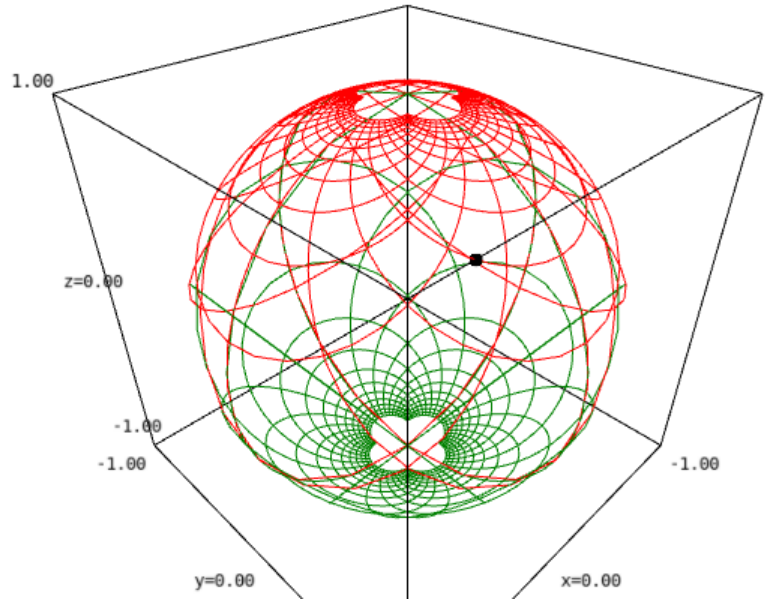
\includegraphics[width=0.8\textwidth]{sphere_stereo.png}
\end{center}

%%%%%%%%%%%%%%%%%%%%%%%%%%%%%%%%%%%%%%%%%%%%%%%%%%%%%%%%%%%%%%%%%%%%%%%%%%%%%%%

\section{Scalar fields and their algebra} \label{s:man:scalar_field_algebra}

\subsection{Definition and implementation} \label{s:man:def_scalar}

Given a smooth manifold $\M$ over a topological field $\K$,
a \defin{scalar field}\index{scalar!field} (also called a
\defin{scalar-valued function}\index{scalar-valued function}) on $\M$
is a smooth map
\be
    \begin{array}{lcll}
    f: & \M &\longrightarrow & \K \\
       & p & \longmapsto  & f(p) .
    \end{array}
\ee
A scalar field has different coordinate representations $F$, $\hat F$, etc.
in different charts $X$, $\hat X$, etc. defined on $M$:
\be \label{e:man:repr_scalar_field}
    f(p) =
F(\underbrace{x^1,\ldots, x^n}_{\mbox{coord. of $p$}\atop\mbox{in chart $X$}})
= {\hat F}(\underbrace{{\hat x}^1,\ldots, {\hat x}^n}_{\mbox{coord. of $p$}\atop\mbox{in chart $\hat X$}})
= \ldots
\ee

In \Sage{}, scalar fields are implemented by the class
\code{DiffScalarField}\footurl{http://doc.sagemath.org/html/en/reference/manifolds/sage/manifolds/differentiable/scalarfield.html}
and the various representations~\eqref{e:man:repr_scalar_field} are
stored in the private attribute \code{\_express} of this class, which is a
Python dictionary
whose keys are the various charts defined on $M$:
\be \label{e:f_express}
 f.\mbox{\texttt{\_express}} = \left\{ X: F,\ \hat X: \hat F, \ldots \right\} .
\ee
Each representation $F$ is an instance of the class \code{ChartFunction},
devoted to functions of coordinates, allowing for different internal representations:
\Sage{} symbolic expression, \soft{SymPy} expression, etc.

For instance, let us define a scalar field on our example manifold $M=\Sp$:
\begin{NBin}
f = M.scalar_field({XU: 1/(1+x^2+y^2), XV: (xp^2+yp^2)/(1+xp^2+yp^2)},
                   name='f')
f.display()
\end{NBin}
\begin{NBoutM}
\begin{array}{llcl} f:& M & \longrightarrow & \mathbb{R} \\ \mbox{on}\ U : & \left(x, y\right) & \longmapsto & \frac{1}{x^{2} + y^{2} + 1} \\ \mbox{on}\ V : & \left({x'}, {y'}\right) & \longmapsto & \frac{{x'}^{2} + {y'}^{2}}{{x'}^{2} + {y'}^{2} + 1} \end{array}
\end{NBoutM}
The internal dictionary \code{\_express} is then
\begin{NBin}
f._express
\end{NBin}
\begin{NBoutM}
\left\{\left(U,(x, y)\right) : \frac{1}{x^{2} + y^{2} + 1}, \left(V,({x'}, {y'})\right) : \frac{{x'}^{2} + {y'}^{2}}{{x'}^{2} + {y'}^{2} + 1}\right\}
\end{NBoutM}
The reader may wonder about the compatibility of the two coordinate expressions
provided in the definition of $f$. Actually, to ensure the compatibility, it
is possible to declare the scalar field in a single chart, \code{XU} say,
and then to obtain its expression in chart \code{XV} by analytic continuation
from the expression in $W=U\cap V$, where both expressions are known, thanks
to the transition map \code{XV}~$\to$~\code{XU}:
\begin{NBin}
f0 = M.scalar_field({XU: 1/(1+x^2+y^2)})
f0.add_expr_by_continuation(XV, U.intersection(V))
f == f0
\end{NBin}
\begin{NBout}
\texttt{True}
\end{NBout}
The representation of the scalar field in a given chart, i.e.\ the public access
to the private directory \code{\_express}, is obtained via the method \code{coord\_function()}:
\begin{NBin}
fU = f.coord_function(XU)
fU.display()
\end{NBin}
\begin{NBoutM}
\left(x, y\right) \mapsto \frac{1}{x^{2} + y^{2} + 1}
\end{NBoutM}
\begin{NBin}
fV = f.coord_function(XV)
fV.display()
\end{NBin}
\begin{NBoutM}
\left({x'}, {y'}\right) \mapsto \frac{{x'}^{2} + {y'}^{2}}{{x'}^{2} + {y'}^{2} + 1}
\end{NBoutM}
As mentioned above, each chart representation is an instance of the
class \code{ChartFunction}:
\begin{NBin}
isinstance(fU, sage.manifolds.chart_func.ChartFunction)
\end{NBin}
\begin{NBout}
\texttt{True}
\end{NBout}
Mathematically, \defin{chart functions}\index{chart!function} are $\K$-valued functions on the codomain of
the considered chart. They map coordinates to elements of the base field $\K$:
\begin{NBin}
fU(1,2)
\end{NBin}
\begin{NBoutM}
\frac{1}{6}
\end{NBoutM}
\begin{NBin}
fU(*XU(p))
\end{NBin}
\begin{NBoutM}
\frac{1}{6}
\end{NBoutM}
Note the use of Python's star operator in \code{*XU(p)} to unpack the tuple of coordinates
returned by \code{XU(p)} (in the present case: \code{(1,2)}) to positional arguments
for the function \code{fU} (in the present case: \code{1, 2}).
On their side, scalar fields map \emph{manifold points}, not coordinates, to $\K$:
\begin{NBin}
f(p)
\end{NBin}
\begin{NBoutM}
\frac{1}{6}
\end{NBoutM}
Note that the equality between \code{Out[32]} and \code{Out[33]}
reflects the identity $f = F \circ X$, where $F$ is the chart function
(denoted \code{fU} above)
representing the scalar field $f$ on the chart $X$
(cf.\ Eq.~\eqref{e:man:repr_scalar_field}).

Internally, each chart function stores coordinate expressions with respect
to various computational engines:
\begin{itemize}
\item \Sage{} symbolic engine, based on the \soft{Pynac}\footnote{\url{http://pynac.org}}\index{Pynac} backend, with \soft{Maxima} used for some simplifications
or computation of integrals;
\item \soft{SymPy}\footnote{\url{http://www.sympy.org}}\index{SymPy} (Python library for symbolic mathematics);
\item in the future, more symbolic or numerical engines will be implemented.
\end{itemize}
The coordinate expressions are stored in the private dictionary \code{\_express}\footnote{not to be confused with
the attribute \code{\_express} of class \code{DiffScalarField} presented
at \code{In~[26]}}
of the class \code{ChartFunction},
whose keys are strings identifying the computational engines. By default
only \Sage{} symbolic expressions, i.e.\ expressions pertaining
to the so-called \Sage{}'s Symbolic Ring (\code{SR}),
are stored:
\begin{NBin}
fU._express
\end{NBin}
\begin{NBoutM}
\left\{\verb|SR| : \frac{1}{x^{2} + y^{2} + 1}\right\}
\end{NBoutM}
The public access to the private dictionary \code{\_express} is performed via the
method \code{expr()}:
\begin{NBin}
fU.expr()
\end{NBin}
\begin{NBoutM}
\frac{1}{x^{2} + y^{2} + 1}
\end{NBoutM}
\begin{NBin}
type(fU.expr())
\end{NBin}
\begin{NBout}
\begin{verbatim}
<type 'sage.symbolic.expression.Expression'>
\end{verbatim}
\end{NBout}
Actually, \code{fU.expr()} is a shortcut for \code{fU.expr('SR')} since
\code{SR} is the default symbolic engine. Note that the class
\code{Expression} is that devoted to \Sage{} symbolic expressions.
The method \code{expr()} can also be invoked to get the expression in
another symbolic engine, for instance \soft{SymPy}:
\begin{NBin}
fU.expr('sympy')
\end{NBin}
\begin{NBout}
\verb|1/(x**2|\phantom{\verb!x!}\verb|+|\phantom{\verb!x!}\verb|y**2|\phantom{\verb!x!}\verb|+|\phantom{\verb!x!}\verb|1)|
\end{NBout}
\begin{NBin}
type(fU.expr('sympy'))
\end{NBin}
\begin{NBout}
\begin{verbatim}
<class 'sympy.core.power.Pow'>
\end{verbatim}
\end{NBout}
This operation has updated the internal dictionary \code{\_express}
(compare with \code{Out~[34]}):
\begin{NBin}
fU._express
\end{NBin}
\begin{NBoutM}
\left\{\texttt{SR} : \frac{1}{x^{2} + y^{2} + 1},
\texttt{sympy}: \mbox{\texttt{1/(x**2 + y**2 + 1)}}\right\}
\end{NBoutM}
The default calculus engine for chart functions of chart \code{XU} can
changed thanks to the method \code{set\_calculus\_method()}:
\begin{NBin}
XU.set_calculus_method('sympy')
fU.expr()
\end{NBin}
\begin{NBout}
\verb|1/(x**2|\phantom{\verb!x!}\verb|+|\phantom{\verb!x!}\verb|y**2|\phantom{\verb!x!}\verb|+|\phantom{\verb!x!}\verb|1)|
\end{NBout}
Reverting to \Sage{}'s symbolic engine:
\begin{NBin}
XU.set_calculus_method('SR')
fU.expr()
\end{NBin}
\begin{NBoutM}
\frac{1}{x^{2} + y^{2} + 1}
\end{NBoutM}
Symbolic expressions can be accessed directly from the scalar field,
\code{f.expr(XU)} being a shortcut for \code{f.coord\_function(XU).expr()}:
\begin{NBin}
f.expr(XU)
\end{NBin}
\begin{NBoutM}
\frac{1}{x^{2} + y^{2} + 1}
\end{NBoutM}
\begin{NBin}
f.expr(XV)
\end{NBin}
\begin{NBoutM}
\frac{{x'}^{2} + {y'}^{2}}{{x'}^{2} + {y'}^{2} + 1}
\end{NBoutM}

\begin{figure}
\begin{center}
\begin{tikzpicture}[font=\small, node distance=0.5cm, minimum
height=2em, auto]

\node[native](unique_representation)
{\code{UniqueRepresentation}};

\node[native, right=of unique_representation](parent)
{\code{Parent}};

\coordinate (Middle) at ($(unique_representation)!0.5!(parent)$);

\node[diff, below=1.5cm of Middle](scalar_field_algebra)
{\code{ScalarFieldAlgebra}\\
{\scriptsize {\it element:} \code{ScalarField}}};
\path[line] (scalar_field_algebra) -- (unique_representation);
\path[line] (scalar_field_algebra) -- node [near start, yshift=-0.5em,
xshift=15.4em]
{\scriptsize {\it category:} \code{CommutativeAlgebras(base\_field)}} (parent);

\node[diff, below=1.25cm of scalar_field_algebra](diff_scalar_field_algebra)
{\code{DiffScalarFieldAlgebra}\\
{\scriptsize {\it element:} \code{DiffScalarField}}};
\path[line] (diff_scalar_field_algebra) -- (scalar_field_algebra);

% Elements:

\node[native, right=3cm of parent](caelement)
{\code{CommutativeAlgebraElement}};

\node[diff, below=1.25cm of caelement](scalarfield)
{\code{ScalarField}\\ \scriptsize{\it parent:} \code{ScalarFieldAlgebra}};
\path[line] (scalarfield) -- (caelement);

\node[diff, below=1.25cm of scalarfield](diff_scalarfield)
{\code{DiffScalarField}\\ \scriptsize{\it parent:} \code{DiffScalarFieldAlgebra}};
\path[line] (diff_scalarfield) -- (scalarfield);


% legend

\node[native_legend, below=0.5cm of diff_scalar_field_algebra]
(native_legend){};
\node[empty, right=0.5em of native_legend]
{Generic \Sage{} class};

\node[diff_legend, below=1.em of native_legend]
(diff_legend){};
\node[empty, right=0.5em of diff_legend]
{\SM{} class\\ \footnotesize (differential part)};

\end{tikzpicture}

\end{center}
\caption{\label{f:man:scalar_classes}\footnotesize
\Sage{} classes for scalar fields on a manifold.}
\end{figure}

\subsection{Scalar field algebra} \label{s:man:scal_algebra}

The set $C^\infty(M)$
of all scalar fields on $M$ has naturally the structure of a
commutative algebra over $\K$: it is clearly a vector
space over $\K$ and it is endowed with a commutative ring structure
by pointwise multiplication:
\be
\forall f, g \in C^\infty(M),\quad \forall p\in M,\quad
(f.g)(p) := f(p) g(p) .
\ee
The algebra $C^\infty(M)$ is implemented in \Sage{} via the parent
class\\ \code{DiffScalarFieldAlgebra},\footurl{http://doc.sagemath.org/html/en/reference/manifolds/sage/manifolds/differentiable/scalarfield_algebra.html} in the category
\code{CommutativeAlgebras}. The corresponding element class
is of course \code{DiffScalarField} (cf.\ Fig.~\ref{f:man:scalar_classes}).

The \Sage{} object representing $C^\infty(M)$ is obtained from \code{M} via the
method\\ \code{scalar\_field\_algebra()}:
\begin{NBin}
CM = M.scalar_field_algebra()
CM
\end{NBin}
\begin{NBoutM}
C^{\infty}\left(M\right)
\end{NBoutM}
\begin{NBin}
CM.category()
\end{NBin}
\begin{NBoutM}
\mathbf{CommutativeAlgebras}_{\text{SR}}
\end{NBoutM}
As for the manifold classes, the actual Python class implementing
$C^\infty(M)$ is inherited from \code{DiffScalarFieldAlgebra} via \Sage{}'s
category framework (cf.\ Sec.~\ref{s:bas:def_manif}), hence it bares the name \code{DiffScalarFieldAlgebra\_with\_category}:
\begin{NBin}
type(CM)
\end{NBin}
\begin{NBout}
\begin{verbatim}
<class 'sage.manifolds.differentiable.scalarfield_algebra.
        DiffScalarFieldAlgebra_with_category'>
\end{verbatim}
\end{NBout}
The class \code{DiffScalarFieldAlgebra\_with\_category} is dynamically generated
as a subclass of \code{DiffScalarFieldAlgebra} with extra functionalities, like
for instance the method \code{is\_commutative()}:
\begin{NBin}
CM.is_commutative()
\end{NBin}
\begin{NBout}
\texttt{True}
\end{NBout}
To have a look at the corresponding code,
we use the double question mark, owing to the fact that \Sage{} is open-source:
\begin{NBin}
CM.is_commutative??
\end{NBin}
\begin{lstlisting}
def is_commutative(self):
    """
    Return ``True``, since commutative magmas are commutative.

    EXAMPLES::

        sage: Parent(QQ,category=CommutativeRings()).is_commutative()
        True
    """
    return True
File: .../local/lib/python2.7/site-packages/sage/categories/magmas.py
\end{lstlisting}
We see from the \code{File} field in line~11 that the code belongs to the category part of \Sage{}, not to the
manifold part, where the class \code{DiffScalarFieldAlgebra} is defined.
This shows that the method \code{is\_commutative()} has indeed be
added to the methods of the base class \code{DiffScalarFieldAlgebra}, while
dynamically generating the class \\ \code{DiffScalarFieldAlgebra-with-category}.

Regarding the scalar field \code{f} introduced in Sec.~\ref{s:man:def_scalar}, we
have of course
\begin{NBin}
f in CM
\end{NBin}
\begin{NBout}
\texttt{True}
\end{NBout}
Actually, in \Sage{} language, \code{CM}=$C^\infty(M)$ is the parent of \code{f}:
\begin{NBin}
f.parent() is CM
\end{NBin}
\begin{NBout}
\texttt{True}
\end{NBout}
The zero element of the algebra $C^\infty(M)$ is
\begin{NBin}
CM.zero().display()
\end{NBin}
\begin{NBoutM}
\begin{array}{llcl} 0:& M & \longrightarrow & \mathbb{R} \\ \mbox{on}\ U : & \left(x, y\right) & \longmapsto & 0 \\ \mbox{on}\ V : & \left({x'}, {y'}\right) & \longmapsto & 0 \end{array}
\end{NBoutM}
while its unit element is
\begin{NBin}
CM.one().display()
\end{NBin}
\begin{NBoutM}
\begin{array}{llcl} 1:& M & \longrightarrow & \mathbb{R} \\ \mbox{on}\ U : & \left(x, y\right) & \longmapsto & 1 \\ \mbox{on}\ V : & \left({x'}, {y'}\right) & \longmapsto & 1 \end{array}
\end{NBoutM}

\subsection{Implementation of algebra operations} \label{s:man:add_implement}

Let us consider some operation in the algebra $C^\infty(M)$:
\begin{NBin}
h = f + 2*CM.one()
h.display()
\end{NBin}
\begin{NBoutM}
\begin{array}{llcl} & M & \longrightarrow & \mathbb{R} \\ \mbox{on}\ U : & \left(x, y\right) & \longmapsto & \frac{2 \, x^{2} + 2 \, y^{2} + 3}{x^{2} + y^{2} + 1} \\ \mbox{on}\ V : & \left({x'}, {y'}\right) & \longmapsto & \frac{3 \, {x'}^{2} + 3 \, {y'}^{2} + 2}{{x'}^{2} + {y'}^{2} + 1} \end{array}
\end{NBoutM}
\begin{NBin}
h(p)
\end{NBin}
\begin{NBoutM}
\frac{13}{6}
\end{NBoutM}
Let us examine how the addition in \code{In~[53]} is performed. For the Python interpreter
\code{h = f + 2*CM.one()} is equivalent to \code{h = f.\_\_add\_\_(2*CM.one())},
i.e.\ the \code{+} operator amounts to calling the method \code{\_\_add\_\_()} on its
left operand, with the right operand as argument.
To have a look at the source code of this method, we use the double question mark:\footnote{In this
transcript of code and in those that follow, some parts
have been skipped, being not relevant for the discussion; they are marked
by ``\code{...}''.}
\begin{NBin}
f.__add__??
\end{NBin}
\label{p:man:list___add__}
\begin{lstlisting}
File: .../src/sage/structure/element.pyx
def __add__(left, right):
    """
    Top-level addition operator for :class:`Element` invoking
    the coercion model.

    See :ref:`element_arithmetic`.
    ...
    """
    cdef int cl = classify_elements(left, right)
    if HAVE_SAME_PARENT(cl):
        return (<Element>left)._add_(right)
    # Left and right are Sage elements => use coercion model
    if BOTH_ARE_ELEMENT(cl):
        return coercion_model.bin_op(left, right, add)
    ...
\end{lstlisting}
From lines 1 and 4, we
see that the method \code{\_\_add\_\_()} is implemented at the level
of the class \code{Element} from which \code{DiffScalarField} inherits, via
\code{CommutativeAlgebraElement} (cf.\ Fig.~\ref{f:man:scalar_classes}).
In the present case, \code{left} = \code{f} and \code{right} = \code{2*CM.one()}
have the same parent, namely the algebra \code{CM}, so that the actual
result is computed in line~12. The latter invokes the method \code{\_add\_()}
(note the single underscore on each side of \code{add}). This operator is
implemented at the level of \code{ScalarField}, as checked from the source code (see line~24 below):
\begin{NBin}
f._add_??
\end{NBin}
\begin{lstlisting}
def _add_(self, other):
    """
    Scalar field addition.

    INPUT:
    - ``other`` -- a scalar field (in the same algebra as ``self``)

    OUTPUT:
    - the scalar field resulting from the addition of ``self`` and
      ``other``
    ...
    """
    ...
    # Generic case:
    com_charts = self.common_charts(other)
    if com_charts is None:
        raise ValueError("no common chart for the addition")
    result = type(self)(self.parent())
    for chart in com_charts:
        # ChartFunction addition:
        result._express[chart] = self._express[chart] + other._express[chart]
    ...
    return result
File: .../local/lib/python2.7/site-packages/sage/manifolds/scalarfield.py
\end{lstlisting}
This reflects a general strategy\footnote{See \url{http://doc.sagemath.org/html/en/thematic_tutorials/coercion_and_categories.html} for details.} in \Sage{}: the arithmetic Python operators
\code{\_\_add\_\_()}, \code{\_\_sub\_\_()}, etc. are implemented at the
top-level class \code{Element}, while specific element subclasses,
like \code{ScalarField} here, implement single-underscore methods
\code{\_add\_()}, \code{\_sub\_()}, etc., which perform the actual computation
when both operands have the same parent.
Looking at the code (lines~15 to 23), we notice that the first step is to search
for the charts in which both operands of the addition operator have a coordinate
expression (line~15). This is performed by the method \code{common\_charts()};
in the current example, we get the two stereographic charts defined on $M$:
\begin{NBin}
f.common_charts(2*CM.one())
\end{NBin}
\begin{NBoutM}
\left[\left(U,(x, y)\right), \left(V,({x'}, {y'})\right)\right]
\end{NBoutM}
In general, \code{common\_charts()} returns the charts for which both operands
have already a known coordinate expression or for which a coordinate
expression can be computed by a known transition map, as we can see on the source
code:
\begin{NBin}
f.common_charts??
\end{NBin}
\begin{lstlisting}
def common_charts(self, other):
    """
    Find common charts for the expressions of the scalar field and
    ``other``.

    INPUT:
    - ``other`` -- a scalar field

    OUTPUT:
    - list of common charts; if no common chart is found, ``None`` is
      returned (instead of an empty list)
    ...
    """
    if not isinstance(other, ScalarField):
        raise TypeError("the second argument must be a scalar field")
    coord_changes = self._manifold._coord_changes
    resu = []
    #
    # 1/ Search for common charts among the existing expressions, i.e.
    #    without performing any expression transformation.
    #    -------------------------------------------------------------
    for chart1 in self._express:
        if chart1 in other._express:
            resu.append(chart1)
    # Search for a subchart:
    known_expr1 = self._express.copy()
    known_expr2 = other._express.copy()
    for chart1 in known_expr1:
        if chart1 not in resu:
            for chart2 in known_expr2:
                if chart2 not in resu:
                    if chart2 in chart1._subcharts:
                        self.expr(chart2)
                        resu.append(chart2)
                    if chart1 in chart2._subcharts:
                        other.expr(chart1)
                        resu.append(chart1)
    #
    # 2/ Search for common charts via one expression transformation
    #    ----------------------------------------------------------
    for chart1 in known_expr1:
        if chart1 not in resu:
            for chart2 in known_expr2:
                if chart2 not in resu:
                    if (chart1, chart2) in coord_changes:
                        self.coord_function(chart2, from_chart=chart1)
                        resu.append(chart2)
                    if (chart2, chart1) in coord_changes:
                        other.coord_function(chart1, from_chart=chart2)
                        resu.append(chart1)
    if resu == []:
        return None
    else:
        return resu
File: .../local/lib/python2.7/site-packages/sage/manifolds/scalarfield.py
\end{lstlisting}
Once the list of charts in which both operands have a coordinate expression
has been found,
the addition is performed at the chart function level (cf.\ Sec.~\ref{s:man:def_scalar}),
via the loop on the charts in lines~19-21 of the code for \code{\_add\_()}.
The code for the addition of chart functions defined on the same chart
is (recall that \code{fU} is the chart function representing $f$ in chart \code{XU}):
\begin{NBin}
fU._add_??
\end{NBin}
\begin{lstlisting}
def _add_(self, other):
    """
    Addition operator.

    INPUT:
    - ``other`` -- a :class:`ChartFunction` or a value

    OUTPUT:
    - chart function resulting from the addition of ``self``
      and ``other``
    ...
    """
    curr = self._calc_method._current
    res = self._simplify(self.expr() + other.expr())
    if curr =='SR' and res.is_trivial_zero():
        # NB: "if res == 0" would be too expensive (cf. #22859)
        return self.parent().zero()
    else:
        return type(self)(self.parent(), res)
File: .../local/lib/python2.7/site-packages/sage/manifolds/chart_func.py
\end{lstlisting}
We notice that the addition is performed in line~14 on the symbolic expression
with respect to the symbolic engine currently at work (\Sage{}/\soft{Pynac}, \soft{SymPy}, ...), as returned by
the method \code{expr()} (see Sec.~\ref{s:man:def_scalar}).
Let us recall that the user can change the symbolic engine at any time
by means of the method \code{set\_calculus\_method()}, applied either to
a chart or to an open subset (possibly \code{M} itself).
Besides, we notice on line~14 above that the result of the symbolic addition
is automatically simplified, by means of the method \code{\_simplify}.
The latter invokes a chain of simplifying functions, which depends on the
symbolic engine.\footnote{See
\url{https://github.com/sagemath/sage/blob/develop/src/sage/manifolds/utilities.py}
for details; note that the simplifications regarding the \soft{SymPy} engine are not
fully implemented yet.}

Let us now discuss the second case in the \code{\_\_add\_\_()} method of
\code{Element}, namely the case for which the parents of both operands are
different (lines~14-15 in the code listed as a result of \code{In [55]},
on page~\pageref{p:man:list___add__}). This case is treated via \Sage{} coercion\index{coercion} model, which allows one to deal with additions like
\begin{NBin}
h1 = f + 2
h1.display()
\end{NBin}
\begin{NBoutM}
\begin{array}{llcl} & M & \longrightarrow & \mathbb{R} \\ \mbox{on}\ U : & \left(x, y\right) & \longmapsto & \frac{2 \, x^{2} + 2 \, y^{2} + 3}{x^{2} + y^{2} + 1} \\ \mbox{on}\ V : & \left({x'}, {y'}\right) & \longmapsto & \frac{3 \, {x'}^{2} + 3 \, {y'}^{2} + 2}{{x'}^{2} + {y'}^{2} + 1} \end{array}
\end{NBoutM}
A priori, \code{f + 2} is not a well defined operation, since the integer $2$ does not
belong to the algebra $C^\infty(M)$. However \Sage{} manages to treat it
because $2$ can be coerced (i.e.\ automatically and unambiguously converted) via \code{CM(2)}
into a element of $C^\infty(M)$, namely the constant scalar field whose value is $2$:
\begin{NBin}
CM(2).display()
\end{NBin}
\begin{NBoutM}
\begin{array}{llcl} & M & \longrightarrow & \mathbb{R} \\ \mbox{on}\ U : & \left(x, y\right) & \longmapsto & 2 \\ \mbox{on}\ V : & \left({x'}, {y'}\right) & \longmapsto & 2 \end{array}
\end{NBoutM}
This happens because there exists a coercion map from the parent of $2$, namely the ring of integers $\mathbb{Z}$
(denoted \code{ZZ} in \Sage{}), to $C^\infty(M)$:
\begin{NBin}
2.parent()
\end{NBin}
\begin{NBoutM}
\mathbf{Z}
\end{NBoutM}
\begin{NBin}
CM.has_coerce_map_from(ZZ)
\end{NBin}
\begin{NBout}
\texttt{True}
\end{NBout}
